%%%%%%%%%%%%%%%%%%%%%%%%%%%%%%%%%%%%%%%%%
% Beamer Presentation
% LaTeX Template
% Version 1.0 (10/11/12)
%
% This template has been downloaded from:
% http://www.LaTeXTemplates.com
%
% License:
% CC BY-NC-SA 3.0 (http://creativecommons.org/licenses/by-nc-sa/3.0/)
%
%%%%%%%%%%%%%%%%%%%%%%%%%%%%%%%%%%%%%%%%%

%----------------------------------------------------------------------------------------
%	PACKAGES AND THEMES
%----------------------------------------------------------------------------------------

\documentclass{beamer}

\mode<presentation> {

% The Beamer class comes with a number of default slide themes
% which change the colors and layouts of slides. Below this is a list
% of all the themes, uncomment each in turn to see what they look like.

%\usetheme{default}
%\usetheme{AnnArbor}
%\usetheme{Antibes}
%\usetheme{Bergen}
% \usetheme{Berkeley}
%\usetheme{Berlin}
%\usetheme{Boadilla}
\usetheme{CambridgeUS}
%\usetheme{Copenhagen}
% \usetheme{Darmstadt}
%\usetheme{Dresden}
% \usetheme{Frankfurt}
%\usetheme{Goettingen}
%\usetheme{Hannover}
%\usetheme{Ilmenau}
%\usetheme{JuanLesPins}
%\usetheme{Luebeck}
% \usetheme{Madrid}
%\usetheme{Malmoe}
%\usetheme{Marburg}
%\usetheme{Montpellier}
% \usetheme{PaloAlto}
%\usetheme{Pittsburgh}
%\usetheme{Rochester}
%\usetheme{Singapore}
%\usetheme{Szeged}
%\usetheme{Warsaw}

% As well as themes, the Beamer class has a number of color themes
% for any slide theme. Uncomment each of these in turn to see how it
% changes the colors of your current slide theme.

% \usecolortheme{albatross}
% \usecolortheme{beaver}
% \usecolortheme{beetle}
%\usecolortheme{crane}
\usecolortheme{dolphin}
%\usecolortheme{dove}
% \usecolortheme{fly}
%\usecolortheme{lily}
% \usecolortheme{orchid}
% \usecolortheme{rose}
% \usecolortheme{seagull}
% \usecolortheme{seahorse}
% \usecolortheme{whale}
% \usecolortheme{wolverine}

%\setbeamertemplate{footline} % To remove the footer line in all slides uncomment this line
%\setbeamertemplate{footline}[page number] % To replace the footer line in all slides with a simple slide count uncomment this line

%\setbeamertemplate{navigation symbols}{} % To remove the navigation symbols from the bottom of all slides uncomment this line
}

\usepackage{graphicx} % Allows including images
\usepackage{booktabs} % Allows the use of \toprule, \midrule and \bottomrule in tables
\usepackage{amsmath}
\usepackage{amsthm}
\usepackage{xcolor}
\usepackage{graphicx}
\usepackage{amsfonts}
\usepackage{amssymb}
\usepackage {tikz}
\usepackage{caption}
\usepackage{subcaption}
\usepackage{circuitikz}
\usepackage {xcolor}
\usepackage{wasysym}
\usepackage[lined]{algorithm2e}
\usepackage{bibentry}
\usetikzlibrary{graphs,graphs.standard}
\setbeamercovered{transparent=8}
\usetikzlibrary{positioning}
% \shorthandoff{=}
%----------------------------------------------------------------------------------------
%	TITLE PAGE
%----------------------------------------------------------------------------------------

\title[Random Spanning Trees]{Random Spanning Trees} % The short title appears at the bottom of every slide, the full title is only on the title page

\author{Bhishmaraj S} % Your name
\institute[CMI] % Your institution as it will appear on the bottom of every slide, may be shorthand to save space
{
Chennai Mathematical Institute \\ % Your institution for the title page
\medskip
\textit{bhishma@cmi.ac.in} % Your email address
}
\date{\today} % Date, can be changed to a custom date

\begin{document}

\begin{frame}
\titlepage % Print the title page as the first slide
\end{frame}

\begin{frame}
\frametitle{Overview} % Table of contents slide, comment this block out to remove it
\tableofcontents % Throughout your presentation, if you choose to use \section{} and \subsection{} commands, these will automatically be printed on this slide as an overview of your presentation
\end{frame}

%----------------------------------------------------------------------------------------
%	PRESENTATION SLIDES
%----------------------------------------------------------------------------------------

%------------------------------------------------
\section{Introduction} % Sections can be created in order to organize your presentation into discrete blocks, all sections and subsections are automatically printed in the table of contents as an overview of the talk
%------------------------------------------------

\subsection{Problem Definition} % A subsection can be created just before a set of slides with a common theme to further break down your presentation into chunks

\begin{frame}
\frametitle{Problem Definition}
% \begin{block}

 Given an undirected connected graph $G = (V, E)$, sample a spanning tree $T$ with probability $\frac{1}{|\mathcal{T}|}$ where $\mathcal{T}$ denotes the set of all spanning trees of $G$. 
 
 We are interested in sampling a tree 
%  
% \end{block}

% \begin{block}

% \onslide<2->{

\end{frame}

\begin{frame}

\frametitle{Applications}
 
Sampling spanning trees happens to be a primitive used in various problems in TCS such as 

\begin{itemize}
\pause
\item Constructing expanders (\cite{10.5555/1496770.1496834}, \cite{doi:10.1137/120890971})
\pause
\item Approximation algorithms for the travelling salesman problem(\cite{6108216}, \cite{doi:10.1287/opre.2017.1603})
\pause
\item Graph Sparcification (\cite{DBLP:journals/corr/abs-1005-0265}, \cite{dolev2016random})
\pause
\item Analysis of network reliability (\cite{10.5555/535891},\cite{doi:10.1002/net.3230200303}, \cite{colbourn1988estimating})
\pause
\item Sequence shuffling problem in Bioinformatics (\cite{KANDEL1996171})
\pause
\item Maze Generation
\end{itemize}
% 
% }
% \end{block}



\end{frame}

%------------------------------------------------

\subsection{Algorithms}
\begin{frame}
 \frametitle{Proposed Algorithms}
 
 In this talk we would review some of the algorithms proposed for this problem and get into details of \cite{harvey2016generating}d
 
\end{frame}


\begin{frame}
\centering
 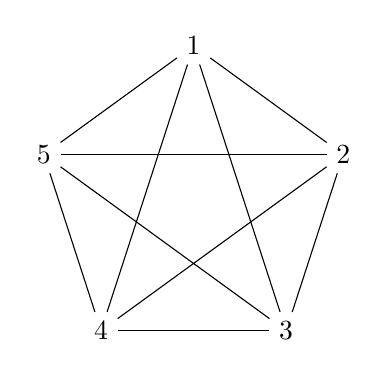
\begin{tikzpicture}
  \graph { subgraph K_n [n=5,clockwise,radius=2cm] };
\end{tikzpicture}
\end{frame}


\begin{frame}
\frametitle{Naive algorithm using effective resistance}


\begin{figure}

\begin{algorithm}[H]
 \KwIn{$G = (V,E) \  \text{and} \  L_G^+$}
 \KwOut{Set of edges corresponding to a random spanning tree}
 
 \For{$e = (u,v) \in E$ }{
    $R_e^{\text{eff}} = (\chi_u - \chi_v)^T \ L_G^+ \ (\chi_u - \chi_v)$\;
  \eIf{$(X \sim \text{Bernoulli}(R_e^{\text{eff}})) = 1$} {
   Add edge $e$ to the spanning tree\;
   $G = G / e$\;
   }{
   $G = G \setminus e$ \;
  }
  Update $ L_G^+ $ \;
 }
 \caption{Sampling uniform spanning tree using chain rule}
\end{algorithm}
 
\end{figure}


\end{frame}

\begin{frame}
\begin{figure}

\centering
 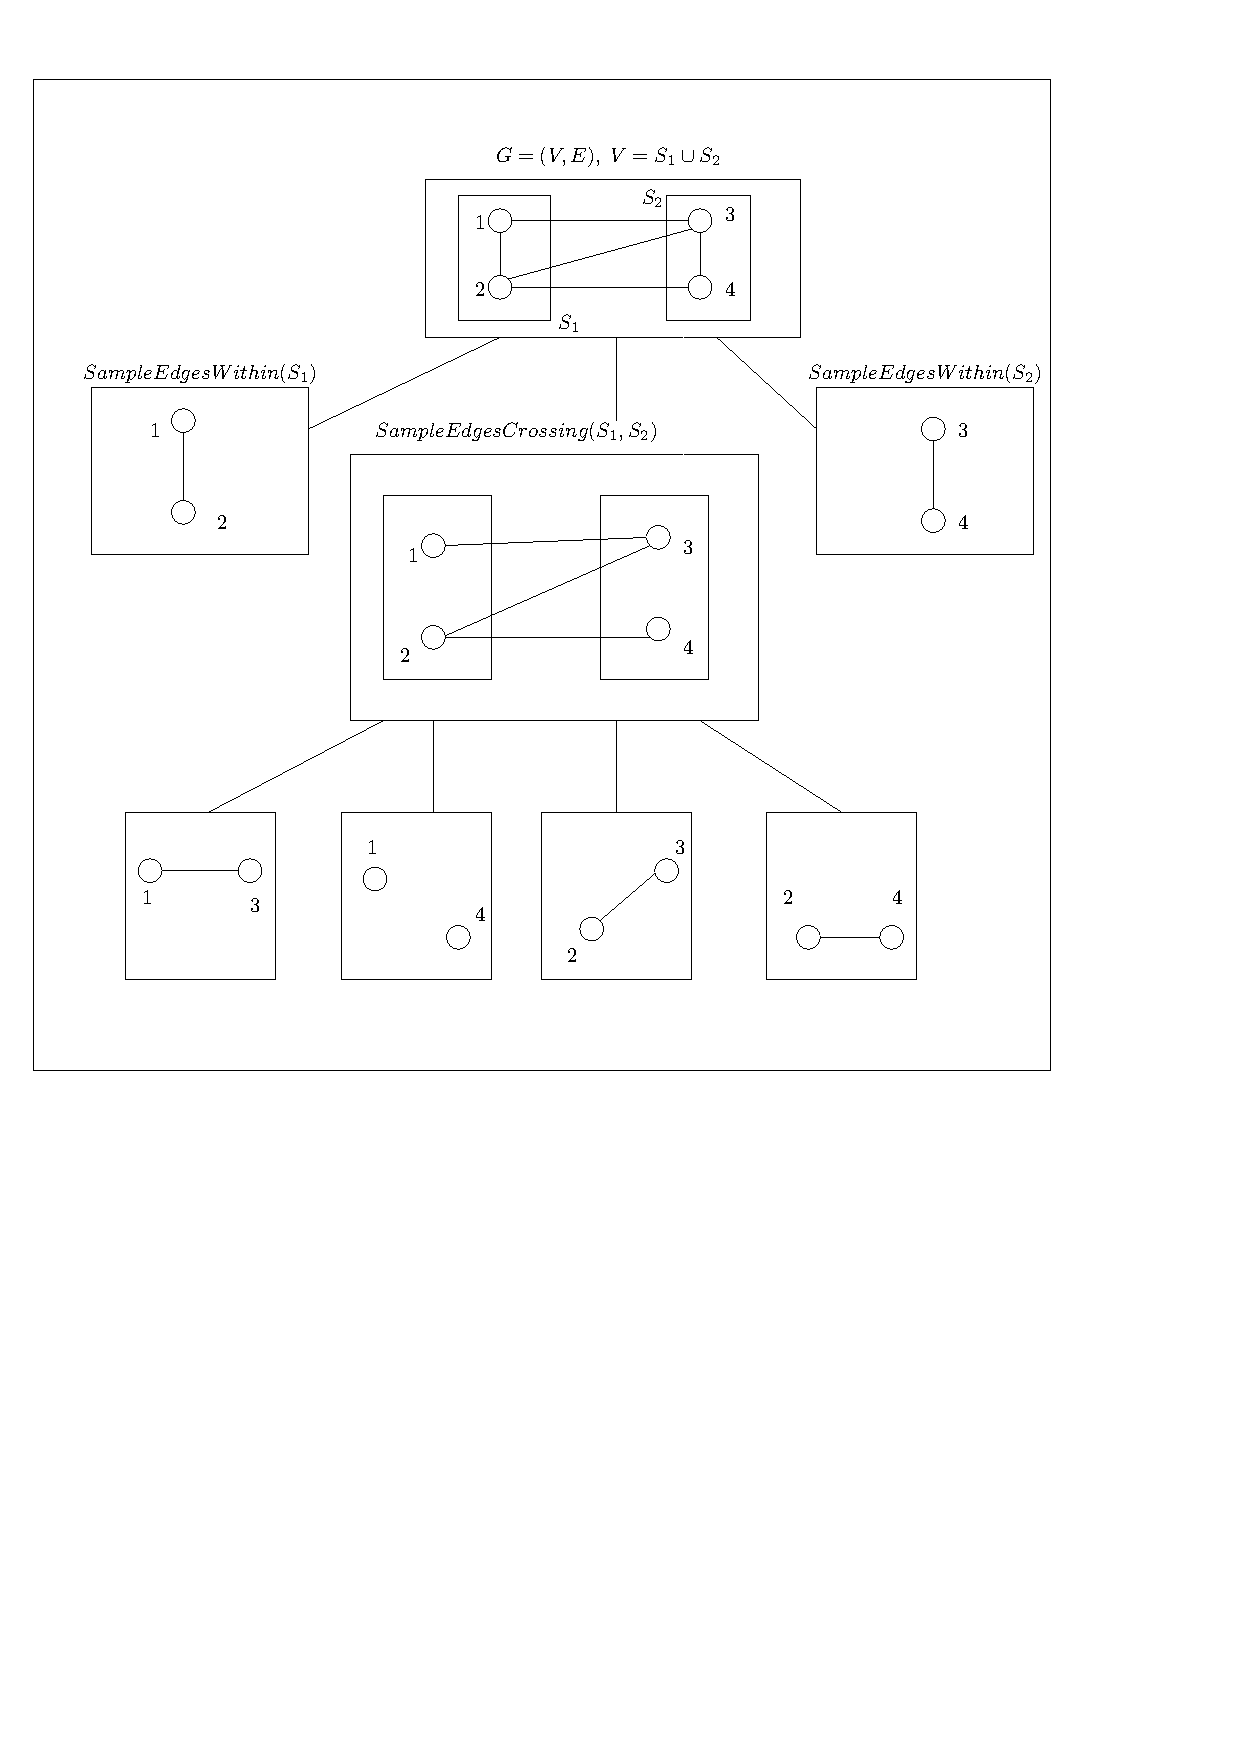
\includegraphics[scale=0.5]{alg-tree}
 
\end{figure}
\end{frame}


%------------------------------------------------

\begin{frame}
\frametitle{Blocks of Highlighted Text}
\pause
\begin{block}{Block 1}
Lorem ipsum dolor sit amet, consectetur adipiscing elit. Integer lectus nisl, ultricies in feugiat rutrum, porttitor sit amet augue. Aliquam ut tortor mauris. Sed volutpat ante purus, quis accumsan dolor.
\end{block}
\pause
\begin{block}{Block 2}
Pellentesque sed tellus purus. Class aptent taciti sociosqu ad litora torquent per conubia nostra, per inceptos himenaeos. Vestibulum quis magna at risus dictum tempor eu vitae velit.
\end{block}
\pause
\begin{block}{Block 3}
Suspendisse tincidunt sagittis gravida. Curabitur condimentum, enim sed venenatis rutrum, ipsum neque consectetur orci, sed blandit justo nisi ac lacus.
\end{block}
\end{frame}

%------------------------------------------------

\begin{frame}
\frametitle{Multiple Columns}
\begin{columns}[c] % The "c" option specifies centered vertical alignment while the "t" option is used for top vertical alignment

\column{.45\textwidth} % Left column and width
\textbf{Heading}
\begin{enumerate}
\item Statement
\item Explanation
\item Example
\end{enumerate}

\column{.5\textwidth} % Right column and width
Lorem ipsum dolor sit amet, consectetur adipiscing elit. Integer lectus nisl, ultricies in feugiat rutrum, porttitor sit amet augue. Aliquam ut tortor mauris. Sed volutpat ante purus, quis accumsan dolor.

\end{columns}
\end{frame}

%------------------------------------------------
\section{Second Section}
%------------------------------------------------

\begin{frame}
\frametitle{Table}
\begin{table}
\begin{tabular}{l l l}
\toprule
\textbf{Treatments} & \textbf{Response 1} & \textbf{Response 2}\\
\midrule
Treatment 1 & 0.0003262 & 0.562 \\
Treatment 2 & 0.0015681 & 0.910 \\
Treatment 3 & 0.0009271 & 0.296 \\
\bottomrule
\end{tabular}
\caption{Table caption}
\end{table}
\end{frame}

%------------------------------------------------

\begin{frame}
\frametitle{Theorem}
\begin{theorem}[Mass--energy equivalence]
$E = mc^2$
\end{theorem}
\end{frame}

%------------------------------------------------

\begin{frame}[fragile] % Need to use the fragile option when verbatim is used in the slide
\frametitle{Verbatim}
\begin{example}[Theorem Slide Code]
\begin{verbatim}
\begin{frame}
\frametitle{Theorem}
\begin{theorem}[Mass--energy equivalence]
$E = mc^2$
\end{theorem}
\end{frame}\end{verbatim}
\end{example}
\end{frame}

%------------------------------------------------
\definecolor {processblue}{cmyk}{0,0,0,0}

\begin{frame}[t]
\frametitle{Figure}

\begin{figure}[h!]
\centering

\begin{subfigure}{.5\textwidth}
  \centering
%   \includegraphics[width=.4\linewidth]{image1}

\begin {tikzpicture}[auto ,node distance =4 cm and 5cm ,on grid ,
semithick ,
state/.style ={ circle ,top color =white , bottom color = processblue!20 ,
draw,black , text=black , minimum width =1 cm}]
\node[state] (C){$A$};
\node[state] (A) [above =of C] {$D$};
\node[state] (B) [above right =of C] {$C$};
\node[state] (D) [right =of C] {$B$};
\path (C) edge node[below] {$1$} (D);
\path (B) edge node[right] {$5$} (D);
\path (A) edge node[above] {$10$} (B);
\path (C) edge node[left] {$4$} (A);
\end{tikzpicture}

  \caption{The original graph $G$}
  \label{fig:sub1}
\end{subfigure}%
\begin{subfigure}{.5\textwidth}
  \centering
%   \includegraphics[width=.4\linewidth]{image1}

\onslide<2->{
\begin{circuitikz}[american]
 \put(0,0){0};
 \draw (0, -2) to[short, -*, i=$1 A$] (0,0) node[left]{$A$};
 \draw (0,0) to[R, l=\mbox{$1 \  \Omega$}] (3,0) node[right]{$B$};
 \draw (0,0) to[R, l=$0.25 \ \Omega$] (0,3) node[left]{$D$};
 \draw (3,0) to[R, l=\mbox{$0.2 \ \Omega$}] (3,3) node[right]{$C$};
 % this works, but it has wrong spacing
 \draw (0,3) to[R, l=$0.1 \ \Omega$] (3,3);
 \draw (3, 0) to[short, *-, i=$1 A$] (3,-2);
 \draw (3, -2) to[isource, l=$1 A$] (0, -2);
 \end{circuitikz}

\caption{The electric network version of $G$}
}
\label{fig:sub2}
\end{subfigure}
\caption{An example of a graph and it's corresponding electric network}
\label{fig:test}
\end{figure}

\end{frame}

%------------------------------------------------

\begin{frame}[fragile] % Need to use the fragile option when verbatim is used in the slide
\frametitle{Aldous-Broder Algorithm example}

\only<1>{
\begin{figure}
\centering
\begin {tikzpicture}[auto ,node distance =4 cm and 5cm ,on grid ,
semithick ,
state/.style ={ circle  , 
draw,black , text=black , minimum width =1 cm}]
\node[state] (C){$C$};
\node[state, fill=white!50!green] (A) [above =of C] {$A$};
\node[state] (B) [above right =of C] {$B$};
\node[state] (D) [right =of C] {$D$};
\path (C) edge[very thick] (D);
\path (B) edge[very thick] (D);
\path (A) edge[very thick] (B);
\path (C) edge[very thick] (A);
\path (D) edge[very thick] (A);
\end{tikzpicture}
 
\end{figure}
}

\only<2>{
\begin{figure}
\centering
\begin {tikzpicture}[auto ,node distance =4 cm and 5cm ,on grid ,
semithick ,
state/.style ={ circle  , 
draw,black , text=black , minimum width =1 cm}]
\node[state] (C){$C$};
\node[state, fill=white!50!red] (A) [above =of C] {$A$};
\node[state, fill=white!50!green] (B) [above right =of C] {$B$};
\node[state] (D) [right =of C] {$D$};
\path (C) edge[very thick] (D);
\path (B) edge[very thick] (D);
\path (A) edge[very thick,blue] (B);
\path (C) edge[very thick] (A);
\path (D) edge[very thick] (A);
\end{tikzpicture}
 
\end{figure}
}

\only<3>{
\begin{figure}
\centering
\begin {tikzpicture}[auto ,node distance =4 cm and 5cm ,on grid ,
semithick ,
state/.style ={ circle  , 
draw,black , text=black , minimum width =1 cm}]
\node[state] (C){$C$};
\node[state, fill=white!50!green] (A) [above =of C] {$A$};
\node[state, fill=white!50!red] (B) [above right =of C] {$B$};
\node[state] (D) [right =of C] {$D$};
\path (C) edge[very thick] (D);
\path (B) edge[very thick] (D);
\path (A) edge[very thick,blue] (B);
\path (C) edge[very thick] (A);
\path (D) edge[very thick] (A);
\end{tikzpicture}
 
\end{figure}
}

\only<4>{
\begin{figure}
\centering
\begin {tikzpicture}[auto ,node distance =4 cm and 5cm ,on grid ,
semithick ,
state/.style ={ circle  , 
draw,black , text=black , minimum width =1 cm}]
\node[state] (C){$C$};
\node[state, fill=white!50!red] (A) [above =of C] {$A$};
\node[state, fill=white!50!red] (B) [above right =of C] {$B$};
\node[state, fill=white!50!green] (D) [right =of C] {$D$};
\path (C) edge[very thick] (D);
\path (B) edge[very thick] (D);
\path (A) edge[very thick,blue] (B);
\path (C) edge[very thick] (A);
\path (D) edge[very thick, blue] (A);
\end{tikzpicture}
 
\end{figure}
}

\only<5>{
\begin{figure}
\centering
\begin {tikzpicture}[auto ,node distance =4 cm and 5cm ,on grid ,
semithick ,
state/.style ={ circle  , 
draw,black , text=black , minimum width =1 cm}]
\node[state] (C){$C$};
\node[state, fill=white!50!red] (A) [above =of C] {$A$};
\node[state, fill=white!50!green] (B) [above right =of C] {$B$};
\node[state, fill=white!50!red] (D) [right =of C] {$D$};
\path (C) edge[very thick] (D);
\path (B) edge[very thick] (D);
\path (A) edge[very thick,blue] (B);
\path (C) edge[very thick] (A);
\path (D) edge[very thick, blue] (A);
\end{tikzpicture}
 
\end{figure}
}

\only<6>{
\begin{figure}
\centering
\begin {tikzpicture}[auto ,node distance =4 cm and 5cm ,on grid ,
semithick ,
state/.style ={ circle  , 
draw,black , text=black , minimum width =1 cm}]
\node[state] (C){$C$};
\node[state, fill=white!50!red] (A) [above =of C] {$A$};
\node[state, fill=white!50!red] (B) [above right =of C] {$B$};
\node[state, fill=white!50!green] (D) [right =of C] {$D$};
\path (C) edge[very thick] (D);
\path (B) edge[very thick] (D);
\path (A) edge[very thick,blue] (B);
\path (C) edge[very thick] (A);
\path (D) edge[very thick, blue] (A);
\end{tikzpicture}
 
\end{figure}
}

\only<7>{
\begin{figure}
\centering
\begin {tikzpicture}[auto ,node distance =4 cm and 5cm ,on grid ,
semithick ,
state/.style ={ circle  , 
draw,black , text=black , minimum width =1 cm}]
\node[state, fill=white!50!green] (C){$C$};
\node[state, fill=white!50!red] (A) [above =of C] {$A$};
\node[state, fill=white!50!red] (B) [above right =of C] {$B$};
\node[state, fill=white!50!red] (D) [right =of C] {$D$};
\path (C) edge[very thick, blue] (D);
\path (B) edge[very thick] (D);
\path (A) edge[very thick,blue] (B);
\path (C) edge[very thick] (A);
\path (D) edge[very thick, blue] (A);
\end{tikzpicture}
 
\end{figure}
}


\end{frame}

\begin{frame}
 \frametitle{Wilson's algorithm example}
 
 \only<1>{
\begin{figure}
\centering
\begin {tikzpicture}[auto ,
semithick ,
state/.style ={ circle  , 
draw,black , text=black , minimum width =1 cm}]
\node[state] (A){$A$};
\node[state] (B) [above right=of A] {$B$};
\node[state] (C) [right =of B] {$C$};
\node[state] (D) [below right =of A] {$D$};
\node[state] (E) [right =of D] {$E$};
\node[state, fill=white!50!red] (F) [above right =of E] {$F$};

\path (C) edge[very thick] (D);
\path (B) edge[very thick] (D);
\path (A) edge[very thick] (B);
\path (C) edge[very thick] (B);
\path (D) edge[very thick] (A);
\path (D) edge[very thick] (E);
\path (C) edge[very thick] (E);
\path (C) edge[very thick] (F);
\path (F) edge[very thick] (E);
\end{tikzpicture}
 
\end{figure}
}
 
 \only<2>{
 
 Start at $A$ 
\begin{figure}
\centering
\begin {tikzpicture}[auto ,
semithick ,
state/.style ={ circle  , 
draw,black , text=black , minimum width =1 cm}]
\node[state, fill=white!50!green] (A){$A$};
\node[state] (B) [above right=of A] {$B$};
\node[state] (C) [right =of B] {$C$};
\node[state] (D) [below right =of A] {$D$};
\node[state] (E) [right =of D] {$E$};
\node[state, fill=white!50!red] (F) [above right =of E] {$F$};

\path (C) edge[very thick] (D);
\path (B) edge[very thick] (D);
\path (A) edge[very thick] (B);
\path (C) edge[very thick] (B);
\path (D) edge[very thick] (A);
\path (D) edge[very thick] (E);
\path (C) edge[very thick] (E);
\path (C) edge[very thick] (F);
\path (F) edge[very thick] (E);
\end{tikzpicture}
 
\end{figure}
}

 
 \only<3>{
\begin{figure}
\centering
\begin {tikzpicture}[auto ,
semithick ,
state/.style ={ circle  , 
draw,black , text=black , minimum width =1 cm}]
\node[state, fill=white!50!blue] (A){$A$};
\node[state, fill=white!50!green] (B) [above right=of A] {$B$};
\node[state] (C) [right =of B] {$C$};
\node[state] (D) [below right =of A] {$D$};
\node[state] (E) [right =of D] {$E$};
\node[state, fill=white!50!red] (F) [above right =of E] {$F$};

\path (C) edge[very thick] (D);
\path (B) edge[very thick] (D);
\path[->] (A) edge[very thick, blue]  (B);
\path (C) edge[very thick] (B);
\path (D) edge[very thick] (A);
\path (D) edge[very thick] (E);
\path (C) edge[very thick] (E);
\path (C) edge[very thick] (F);
\path (F) edge[very thick] (E);
\end{tikzpicture}
 
\end{figure}
}

 \only<4>{
\begin{figure}
\centering
\begin {tikzpicture}[auto ,
semithick ,
state/.style ={ circle  , 
draw,black , text=black , minimum width =1 cm}]
\node[state, fill=white!50!blue] (A){$A$};
\node[state, fill=white!50!blue] (B) [above right=of A] {$B$};
\node[state,fill=white!50!green] (C) [right =of B] {$C$};
\node[state] (D) [below right =of A] {$D$};
\node[state] (E) [right =of D] {$E$};
\node[state, fill=white!50!red] (F) [above right =of E] {$F$};

\path (C) edge[very thick] (D);
\path (B) edge[very thick] (D);
\path[->] (A) edge[very thick, blue]  (B);
\path[->] (B) edge[very thick, blue] (C);
\path (D) edge[very thick] (A);
\path (D) edge[very thick] (E);
\path (C) edge[very thick] (E);
\path (C) edge[very thick] (F);
\path (F) edge[very thick] (E);
\end{tikzpicture}
 
\end{figure}
}
 \only<5>{
\begin{figure}
\centering
\begin {tikzpicture}[auto ,
semithick ,
state/.style ={ circle  , 
draw,black , text=black , minimum width =1 cm}]
\node[state, fill=white!50!blue] (A){$A$};
\node[state, fill=white!50!blue] (B) [above right=of A] {$B$};
\node[state,fill=white!50!blue] (C) [right =of B] {$C$};
\node[state,fill=white!50!green] (D) [below right =of A] {$D$};
\node[state] (E) [right =of D] {$E$};
\node[state, fill=white!50!red] (F) [above right =of E] {$F$};

\path[->] (C) edge[very thick,blue] (D);
\path (B) edge[very thick] (D);
\path[->] (A) edge[very thick, blue]  (B);
\path[->] (B) edge[very thick, blue] (C);
\path (D) edge[very thick] (A);
\path (D) edge[very thick] (E);
\path (C) edge[very thick] (E);
\path (C) edge[very thick] (F);
\path (F) edge[very thick] (E);
\end{tikzpicture}
 
\end{figure}
}
 \only<6>{
\begin{figure}
\centering
\begin {tikzpicture}[auto ,
semithick ,
state/.style ={ circle  , 
draw,black , text=black , minimum width =1 cm}]
\node[state, fill=white!50!blue] (A){$A$};
\node[state, fill=white!50!green] (B) [above right=of A] {$B$};
\node[state,fill=white!50!blue] (C) [right =of B] {$C$};
\node[state,fill=white!50!blue] (D) [below right =of A] {$D$};
\node[state] (E) [right =of D] {$E$};
\node[state, fill=white!50!red] (F) [above right =of E] {$F$};

\path[->] (C) edge[very thick,blue] (D);
\path[->] (D) edge[very thick,blue] (B);
\path[->] (A) edge[very thick, blue]  (B);
\path[->] (B) edge[very thick, blue] (C);
\path (D) edge[very thick] (A);
\path (D) edge[very thick] (E);
\path (C) edge[very thick] (E);
\path (C) edge[very thick] (F);
\path (F) edge[very thick] (E);
\end{tikzpicture}
 
\end{figure}
}
 \only<7>{
\begin{figure}
\centering
\begin {tikzpicture}[auto ,
semithick ,
state/.style ={ circle  , 
draw,black , text=black , minimum width =1 cm}]
\node[state, fill=white!50!blue] (A){$A$};
\node[state, fill=white!50!blue] (B) [above right=of A] {$B$};
\node[state,fill=white!50!green] (C) [right =of B] {$C$};
\node[state,fill=white!50!blue] (D) [below right =of A] {$D$};
\node[state] (E) [right =of D] {$E$};
\node[state, fill=white!50!red] (F) [above right =of E] {$F$};

\path[->] (C) edge[very thick,blue] (D);
\path[->] (D) edge[very thick,blue] (B);
\path[->] (A) edge[very thick, blue]  (B);
\path[->] (B) edge[very thick, blue] (C);
\path (D) edge[very thick] (A);
\path (D) edge[very thick] (E);
\path (C) edge[very thick] (E);
\path (C) edge[very thick] (F);
\path (F) edge[very thick] (E);
\end{tikzpicture}
 
\end{figure}
}

 \only<8>{
 
 Notice the \textbf{next(C)} has changed from $D$ to $F$. 
 
\begin{figure}
\centering
\begin {tikzpicture}[auto ,
semithick ,
state/.style ={ circle  , 
draw,black , text=black , minimum width =1 cm}]
\node[state, fill=white!50!blue] (A){$A$};
\node[state, fill=white!50!blue] (B) [above right=of A] {$B$};
\node[state,fill=white!50!blue] (C) [right =of B] {$C$};
\node[state,fill=white!50!blue] (D) [below right =of A] {$D$};
\node[state] (E) [right =of D] {$E$};
\node[state, fill=white!50!green] (F) [above right =of E] {$F$};

\path(C) edge[very thick] (D);
\path[->] (D) edge[very thick,blue] (B);
\path[->] (A) edge[very thick, blue]  (B);
\path[->] (B) edge[very thick, blue] (C);
\path (D) edge[very thick] (A);
\path (D) edge[very thick] (E);
\path (C) edge[very thick] (E);
\path[->] (C) edge[very thick, blue] (F);
\path (F) edge[very thick] (E);
\end{tikzpicture}
 
\end{figure}
}

 \only<9>{
 
 Since a vertex already in the tree has been reached (namely $F$), starting from $A$ we trace the successors and set their \textbf{inTree} value to $True$
 
\begin{figure}
\centering
\begin {tikzpicture}[auto ,
semithick ,
state/.style ={ circle  , 
draw,black , text=black , minimum width =1 cm}]
\node[state, fill=white!50!red] (A){$A$};
\node[state, fill=white!50!red] (B) [above right=of A] {$B$};
\node[state,fill=white!50!red] (C) [right =of B] {$C$};
\node[state] (D) [below right =of A] {$D$};
\node[state] (E) [right =of D] {$E$};
\node[state, fill=white!50!red] (F) [above right =of E] {$F$};

\path(C) edge[very thick] (D);
\path[->] (D) edge[very thick,blue] (B);
\path[->] (A) edge[very thick, red]  (B);
\path[->] (B) edge[very thick, red] (C);
\path (D) edge[very thick] (A);
\path (D) edge[very thick] (E);
\path (C) edge[very thick] (E);
\path[->] (C) edge[very thick, red] (F);
\path (F) edge[very thick] (E);
\end{tikzpicture}
 
\end{figure}
}

 \only<10>{
 
 Since $B$, $C$ are already in the tree they will be skipped and now will start at $D$
 
\begin{figure}
\centering
\begin {tikzpicture}[auto ,
semithick ,
state/.style ={ circle  , 
draw,black , text=black , minimum width =1 cm}]
\node[state, fill=white!50!red] (A){$A$};
\node[state, fill=white!50!red] (B) [above right=of A] {$B$};
\node[state,fill=white!50!red] (C) [right =of B] {$C$};
\node[state,fill=white!50!green] (D) [below right =of A] {$D$};
\node[state] (E) [right =of D] {$E$};
\node[state, fill=white!50!red] (F) [above right =of E] {$F$};

\path(C) edge[very thick] (D);
\path[->] (D) edge[very thick,blue] (B);
\path[->] (A) edge[very thick, red]  (B);
\path[->] (B) edge[very thick, red] (C);
\path (D) edge[very thick] (A);
\path (D) edge[very thick] (E);
\path (C) edge[very thick] (E);
\path[->] (C) edge[very thick, red] (F);
\path (F) edge[very thick] (E);
\end{tikzpicture}
 
\end{figure}
}

 \only<11>{
 
 
 
\begin{figure}
\centering
\begin {tikzpicture}[auto ,
semithick ,
state/.style ={ circle  , 
draw,black , text=black , minimum width =1 cm}]
\node[state, fill=white!50!red] (A){$A$};
\node[state, fill=white!50!red] (B) [above right=of A] {$B$};
\node[state,fill=white!50!red] (C) [right =of B] {$C$};
\node[state,fill=white!50!blue] (D) [below right =of A] {$D$};
\node[state,fill=white!50!green] (E) [right =of D] {$E$};
\node[state, fill=white!50!red] (F) [above right =of E] {$F$};

\path(C) edge[very thick] (D);
\path(D) edge[very thick] (B);
\path[->] (A) edge[very thick, red]  (B);
\path[->] (B) edge[very thick, red] (C);
\path (D) edge[very thick] (A);
\path[->] (D) edge[very thick,blue] (E);
\path (C) edge[very thick] (E);
\path[->] (C) edge[very thick, red] (F);
\path (F) edge[very thick] (E);
\end{tikzpicture}
 
\end{figure}
}

 \only<12>{
  Since $C$ is already in the tree, the random walk stops and the algorithm retraces from $D$ and includes the vertices into the tree
\begin{figure}
\centering
\begin {tikzpicture}[auto ,
semithick ,
state/.style ={ circle  , 
draw,black , text=black , minimum width =1 cm}]
\node[state, fill=white!50!red] (A){$A$};
\node[state, fill=white!50!red] (B) [above right=of A] {$B$};
\node[state,fill=white!50!green] (C) [right =of B] {$C$};
\node[state,fill=white!50!blue] (D) [below right =of A] {$D$};
\node[state,fill=white!50!blue] (E) [right =of D] {$E$};
\node[state, fill=white!50!red] (F) [above right =of E] {$F$};

\path(C) edge[very thick] (D);
\path(D) edge[very thick] (B);
\path[->] (A) edge[very thick, red]  (B);
\path[->] (B) edge[very thick, red] (C);
\path (D) edge[very thick] (A);
\path[->] (D) edge[very thick,blue] (E);
\path[->] (E) edge[very thick,blue] (C);
\path[->] (C) edge[very thick, red] (F);
\path (F) edge[very thick] (E);
\end{tikzpicture}
 
\end{figure}
}

 \only<13>{
  Since $C$ is already in the tree, the random walk stops and the algorithm retraces from $D$ and includes the vertices into the tree
\begin{figure}
\centering
\begin {tikzpicture}[auto ,
semithick ,
state/.style ={ circle  , 
draw,black , text=black , minimum width =1 cm}]
\node[state, fill=white!50!red] (A){$A$};
\node[state, fill=white!50!red] (B) [above right=of A] {$B$};
\node[state,fill=white!50!red] (C) [right =of B] {$C$};
\node[state,fill=white!50!red] (D) [below right =of A] {$D$};
\node[state,fill=white!50!red] (E) [right =of D] {$E$};
\node[state, fill=white!50!red] (F) [above right =of E] {$F$};

\path(C) edge[very thick] (D);
\path(D) edge[very thick] (B);
\path[->] (A) edge[very thick, red]  (B);
\path[->] (B) edge[very thick, red] (C);
\path (D) edge[very thick] (A);
\path[->] (D) edge[very thick,red] (E);
\path[->] (E) edge[very thick,red] (C);
\path[->] (C) edge[very thick, red] (F);
\path (F) edge[very thick] (E);
\end{tikzpicture}
 
\end{figure}
}


\end{frame}



% white!50!red
% white!50!green

%------------------------------------------------


\begin{frame}
\centering
\Huge{Thank You}
\begin{figure}
 \centering
 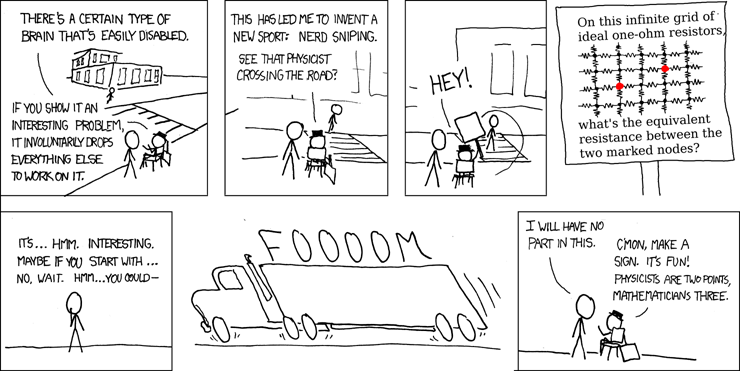
\includegraphics[scale=0.4]{nerd_sniping.png}
 \caption{Obligatory xkcd}
\end{figure}



\end{frame}

% 
% \begin{frame}
% \frametitle{References}
% \footnotesize{
% \begin{thebibliography}{99} % Beamer does not support BibTeX so references must be inserted manually as below
% \bibitem[Smith, 2012]{p1} John Smith (2012)
% \newblock Title of the publication
% \newblock \emph{Journal Name} 12(3), 45 -- 678.
% \end{thebibliography}
% }
% \end{frame}

\begin{frame}
\frametitle{References}
%  \bibliographystyle{amsalpha}
\bibliography{/home/bhishma/Documents/code/masters-thesis/thesis/example.bib}
\end{frame}


%------------------------------------------------

%----------------------------------------------------------------------------------------

\end{document} 
